\chapter{Arquitetura do Sistema}

O sistema desenvolvido adota uma arquitetura moderna e robusta, composta por dois principais componentes: um cliente web desenvolvido com Svelte e um servidor backend implementado em .NET. A comunicação entre cliente e servidor é realizada predominantemente via protocolo HTTP para operações tradicionais de gerenciamento (como criação e entrada em salas de jogo, gerenciamento de contas de usuário e obtenção de dados do jogo). Para operações em tempo real, essenciais para a dinâmica do jogo (como jogar cartas, comprar cartas e receber atualizações instantâneas), utiliza-se o protocolo WebSocket, garantindo baixa latência e interatividade.

\section{Arquitetura em Camadas do Backend}
O backend segue o padrão de arquitetura em camadas, promovendo separação de responsabilidades, facilidade de manutenção e escalabilidade. As principais camadas são:

\begin{itemize}
    \item \textbf{Apresentação}: Responsável por expor as APIs HTTP e WebSocket, recebendo e respondendo às requisições dos clientes. Realiza validações iniciais e orquestra o fluxo das operações.
    \item \textbf{Aplicação}: Contém a lógica de orquestração dos casos de uso do sistema, coordenando as operações entre as demais camadas. Implementa os fluxos de negócio sem se preocupar com detalhes de infraestrutura ou regras de domínio.
    \item \textbf{Domínio}: Abriga as regras de negócio centrais e entidades do sistema. É independente de detalhes técnicos e representa o núcleo lógico da aplicação.
    \item \textbf{Infraestrutura}: Implementa detalhes técnicos como persistência de dados, integração com serviços externos e mecanismos de comunicação. Fornece implementações concretas para interfaces definidas nas camadas superiores.
\end{itemize}

\begin{figure}[H]
    \centering
    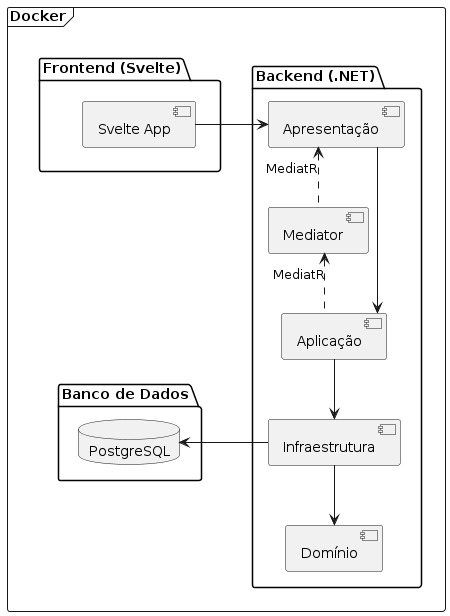
\includegraphics[width=0.7\textwidth]{diagrams/Architecture.png}
    \caption{Diagrama de arquitetura do sistema. Fonte: os autores}
    \label{fig:architecture}
\end{figure}

\section{Padrões de Projeto Utilizados}
O sistema faz uso de alguns padrões de projeto consagrados para promover flexibilidade e desacoplamento:

\begin{enumerate}
    \item \textbf{Repository}: Abstrai o acesso a dados, permitindo que a lógica de negócio interaja com repositórios de forma independente da tecnologia de persistência.
    \item \textbf{Mediator}: Centraliza a comunicação entre componentes, facilitando a implementação de casos de uso e reduzindo o acoplamento entre objetos.
    \item \textbf{Factory}: Facilita a criação de objetos complexos, encapsulando a lógica de instanciação e promovendo flexibilidade na escolha de implementações.
\end{enumerate}

Essa arquitetura garante que o sistema seja modular, testável e preparado para evoluções futuras.

\section{Arquitetura do Frontend}
O frontend do sistema foi desenvolvido utilizando o framework Svelte, que permite a criação de interfaces web reativas e eficientes. A estrutura do projeto segue boas práticas de modularização e separação de responsabilidades, facilitando a manutenção e a escalabilidade da aplicação.

O código-fonte do frontend está organizado em componentes Svelte, cada um responsável por uma parte específica da interface do usuário, como telas de login, gerenciamento de salas, lobby, mesa de jogo e exibição de cartas. Essa abordagem baseada em componentes permite o reuso de código e a fácil evolução da interface.

Além disso, o frontend faz uso de stores reativos do Svelte para gerenciar o estado global da aplicação, como informações do usuário autenticado, estado da sala e dados da partida em andamento. Isso garante que as atualizações de estado sejam refletidas automaticamente na interface, proporcionando uma experiência fluida ao usuário.

A arquitetura adotada no frontend, aliada ao uso de Svelte, resulta em uma aplicação leve, responsiva e de fácil manutenção, preparada para futuras expansões e melhorias.

\section{Tecnologias Utilizadas}
Durante o desenvolvimento do sistema, foram empregadas diversas tecnologias que contribuíram para a robustez, escalabilidade e facilidade de manutenção da solução:

\begin{itemize}
    \item \textbf{SignalR}: Utilizado para facilitar a comunicação em tempo real via WebSocket entre servidor e clientes. O SignalR abstrai a complexidade do gerenciamento de conexões, transmissão de mensagens e reconexão automática, permitindo implementar funcionalidades interativas e síncronas de forma simples e eficiente.
    \item \textbf{MediatR}: Biblioteca empregada para implementar o padrão Mediator no backend, promovendo o desacoplamento entre as camadas de Apresentação e Aplicação. O MediatR centraliza o envio e o tratamento de comandos, queries e eventos, facilitando a manutenção e a evolução do código.
    \item \textbf{PostgreSQL e Entity Framework}: O sistema utiliza o banco de dados relacional PostgreSQL para persistência dos dados, integrado ao backend por meio do Entity Framework, que provê uma camada de abstração para o acesso e manipulação dos dados de forma orientada a objetos.
    \item \textbf{Docker}: Utilizado para empacotar e distribuir tanto o backend quanto o frontend em containers, garantindo portabilidade, reprodutibilidade e facilidade de deploy em diferentes ambientes.
\end{itemize}

Essas tecnologias, integradas à arquitetura do sistema, proporcionam uma base sólida para o desenvolvimento, operação e evolução contínua da aplicação.
